\section{}
\noindent 40. Considere los conjuntos $A = \{(x,y) \in \mathbb{R}^2 : 2 \leq x \leq 3$ y $-1 \leq y < 5\}$ y $B = \{(x,y) \in \mathbb{R}^2 : -2 \leq x < \frac{5}{2}$ y $3 \leq y \leq 7\}$. Describa en el plano cartesiano los conjuntos $A$, $B$ y $A \cap B$.\\

\noindent 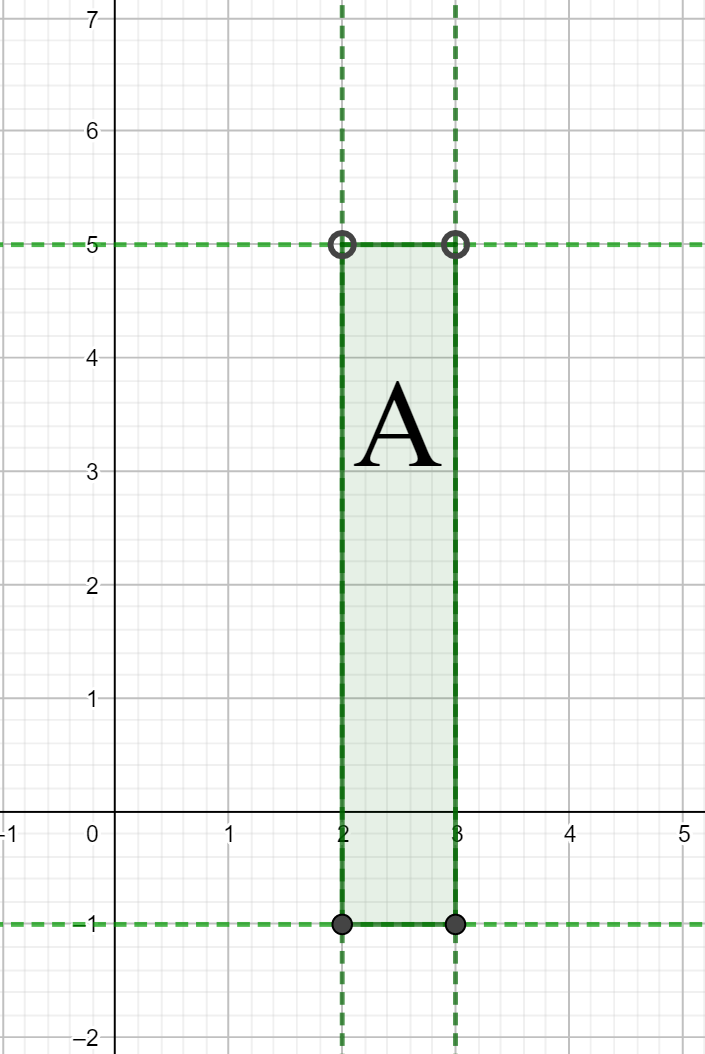
\includegraphics[scale=1]{img/cartesiano_a.png} \indent  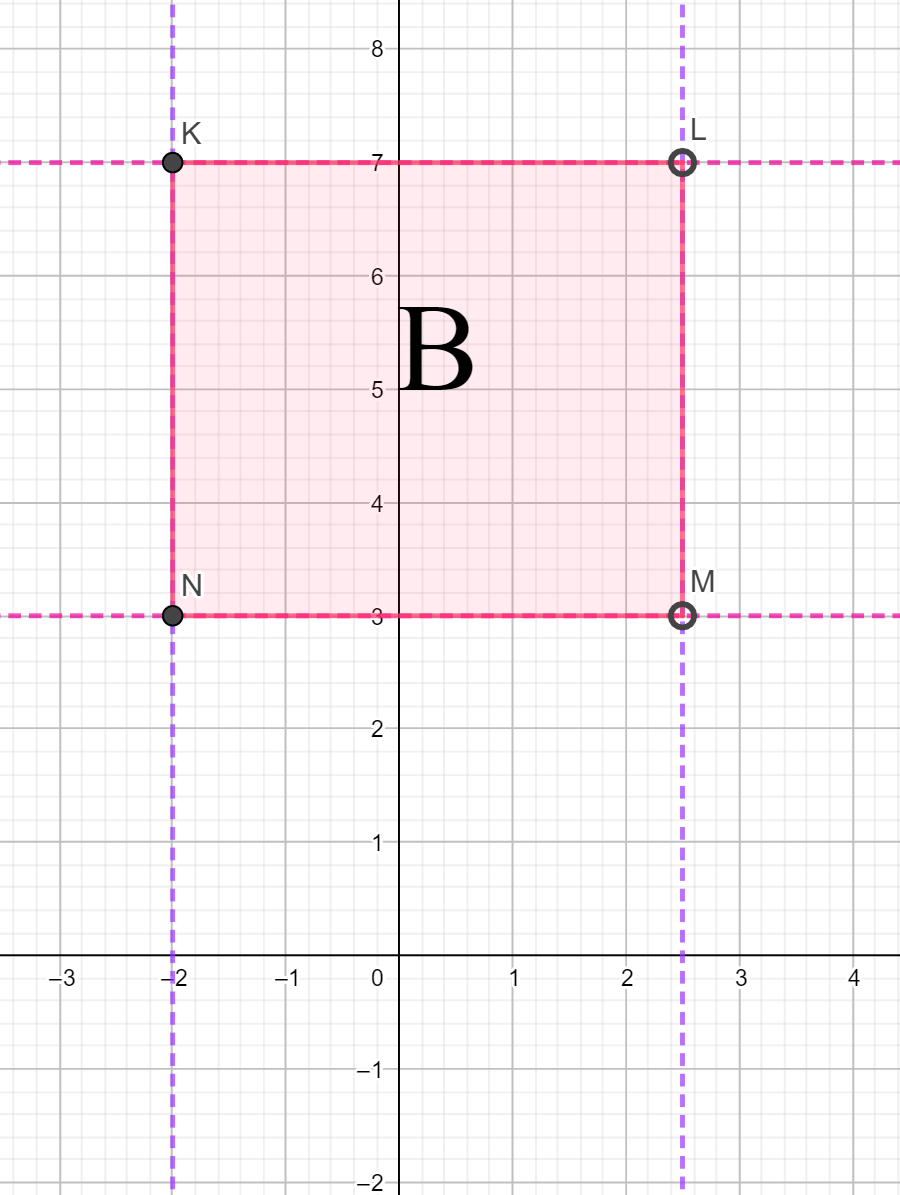
\includegraphics[scale=1]{img/cartesiano_b.png}
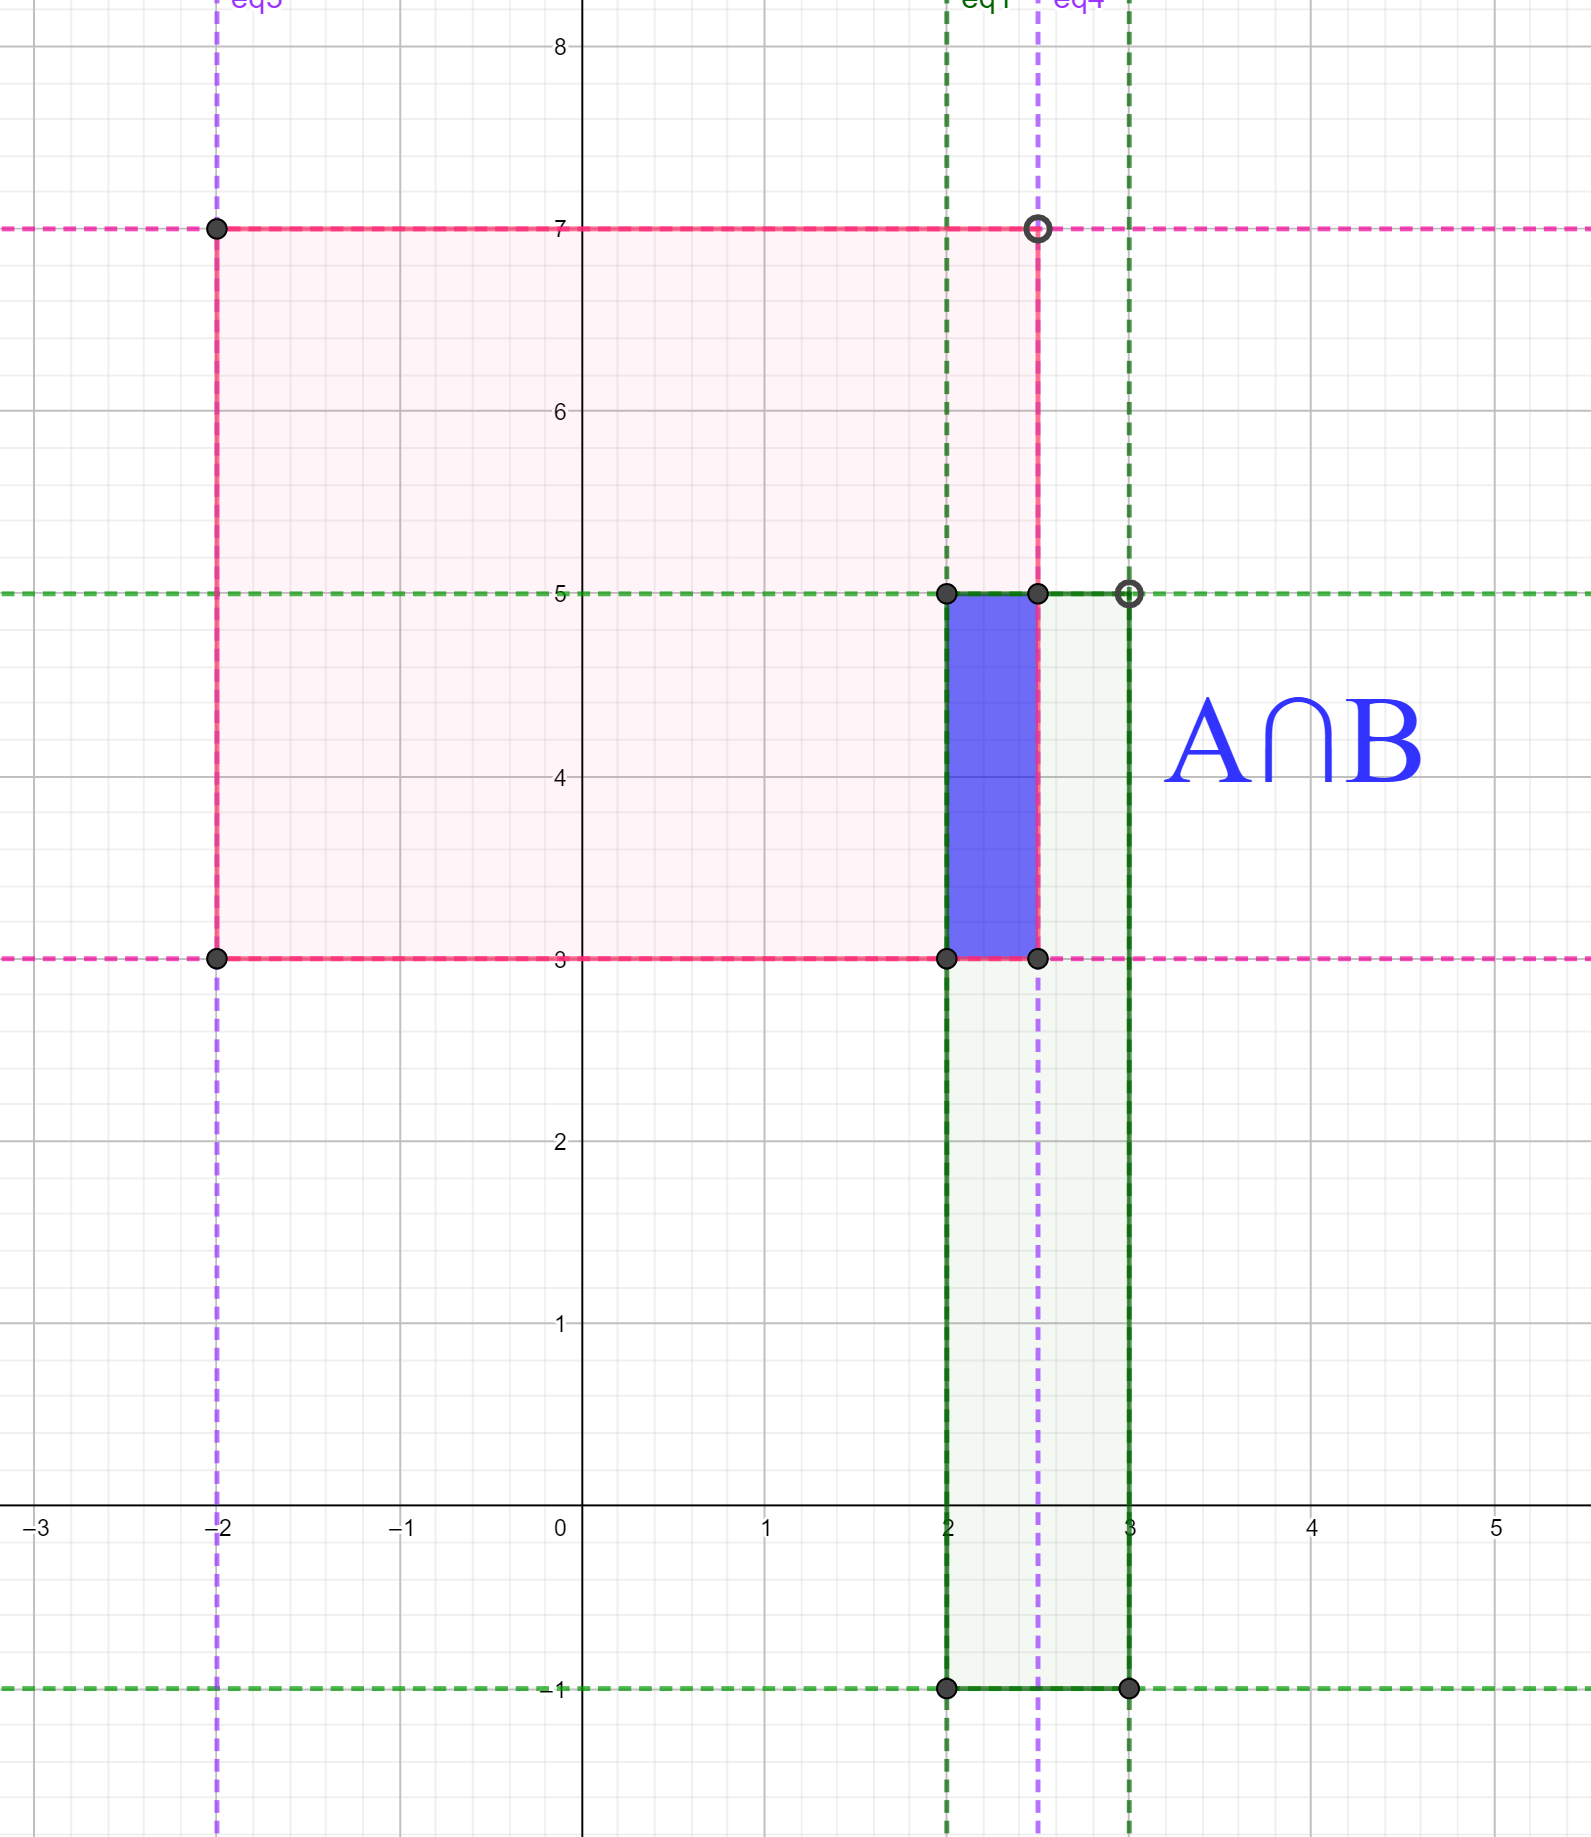
\includegraphics[scale=1]{img/cartesiano_c.png}